\chapter{Cellular Automata}
\label{chapter:cellAuto}
\graphicspath{ {./Lab07CellularAutomata/Fig} }

\section{Outcomes and Objectives}

The outcome of this lab is to instantiate a 1-dimensional
cellular automata using D-Flip Flops and combinational logic.
Through this process you will achieve the following
learning objectives.
\begin{itemize}
    \item \Paste{bok:BasicMemoryElements}
    \item \Paste{bok:BME_Timing}
    \item \Paste{VER:Module}
    \item \Paste{HDL:Synthesis}
\end{itemize}

\section{1-dimensional cellular automata}

A common research theme in intelligent systems is emergent complexity.
This is the idea that complex behavior can arise from an interconnected
arrangement of simple processing elements following simple rules.

\subsection{Theory: Cellular Automata}
As a testbench for this idea, Stephen Wolfram\footnote{Wolfram, S.
    "Statistical Mechanics of Cellular Automata." Rev. Mod. Phys. 55,
601-644, 1983.} explored emergent complexity in a 1-dimensional
cellular automata (1-DCA) network. A 1-DCA is an array of processing
elements, each of which has one of two states (called alive and dead)
and is interconnected to the neighbors immediately to its left and
right. The next state of each processing element depends on its current
state and the current state of the neighbors to its immediate left and
right. Let's explore the evolution of a 1-DCA using the setup shown in
Figure~\ref{fig:exampleCA}, note that cells which are alive are shaded and cells which are
dead, white.

\begin{figure}[ht]
    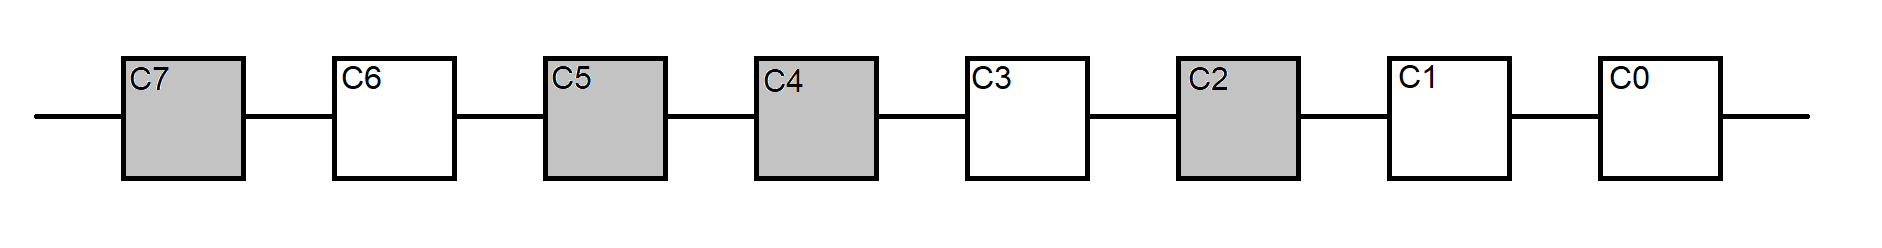
\includegraphics{image1.png}
    \caption{A 1-DCA consisting of 8 processing elements. Alive cells are
    shaded grey, dead white.}
    \label{fig:exampleCA}
\end{figure}

Let's examine the next state of the 1-DCA shown in Figure~\ref{fig:exampleCA}
using the rule where:

\begin{itemize}
    \item
        An alive cell stays alive when exactly 1 of its neighbors is alive,
        else it dies.
    \item
        A dead cell comes alive when exactly 1 of its neighbors is alive, else
        it stays dead.
\end{itemize}

Complete the unfilled entries in Table~\ref{table:caNextState} using the initial state shown
in Figure~\ref{fig:exampleCA} and the rule above. We will imagine that our processing
elements are placed on a ring. This implies that the left neighbor of
processing element C7 is C0 and the right neighbor of processing element
of C0 is C7.

\begin{longtable}[]{@{}
        |  >{\raggedright\arraybackslash}p{(\columnwidth - 6\tabcolsep) * \real{0.1683}}|
        >{\raggedright\arraybackslash}p{(\columnwidth - 6\tabcolsep) * \real{0.2772}}|
        >{\raggedright\arraybackslash}p{(\columnwidth - 6\tabcolsep) * \real{0.3198}}|
    >{\raggedright\arraybackslash}p{(\columnwidth - 6\tabcolsep) * \real{0.2347}}|@{}}
    \caption{The next state of a processing element depends on the
    current state and the number of alive neighbors.} \label{table:caNextState} \tabularnewline
    \toprule()
    \begin{minipage}[b]{\linewidth}\raggedright
        Cell
    \end{minipage} &
    \begin{minipage}[b]{\linewidth}\raggedright
        Current State
    \end{minipage} &
    \begin{minipage}[b]{\linewidth}\raggedright
        \# Alive neighbors
    \end{minipage} &
    \begin{minipage}[b]{\linewidth}\raggedright
        Next State
    \end{minipage} \\
    \midrule()
    \endfirsthead
    \toprule()
    \begin{minipage}[b]{\linewidth}\raggedright
        Cell
    \end{minipage} &
    \begin{minipage}[b]{\linewidth}\raggedright
        Current State
    \end{minipage} &
    \begin{minipage}[b]{\linewidth}\raggedright
        \# Alive neighbors
    \end{minipage} &
    \begin{minipage}[b]{\linewidth}\raggedright
        Next State
    \end{minipage} \\
    \midrule()
    \endhead
    C0 & Dead & & \\ \hline
    C1 & Dead & & \\ \hline
    C2 & Alive & 0 & \\ \hline
    C3 & Dead & & \\ \hline
    C4 & Alive & & Alive \\ \hline
    C5 & Alive & & \\ \hline
    C6 & Dead & & \\ \hline
    C7 & Alive & & \\
    \bottomrule()
\end{longtable}

You are going to build a digital system to calculate the next state of a
9-element array of processing elements. In order to do this, you will
need a way to easily specify the rule used to determine the next state
of a cell because you are going to be able to change it. Before doing
this let's agree to associate the value of 1 for an alive cell and
illustrate it as a filled black square and associate the value 0 with a
dead cell and will illustrate it as an empty square.

We will formalize the next state rule by enumerating the next state of a
cell for every configuration of its current state and its neighbor's
state. Since a cell and it's two neighbors can each have two states,
there are a total of 8 configurations. As an example, I've graphically
illustrated the rule used in our previous example, in Figure~\ref{fig:caRule}. This
arrangement shows the 8 configurations arranged so the binary code of
the current states goes from 3'b000 at right to 3'b111 at left. The next
state for each configuration is shown below the current state
configuration.

\begin{figure}[ht]
    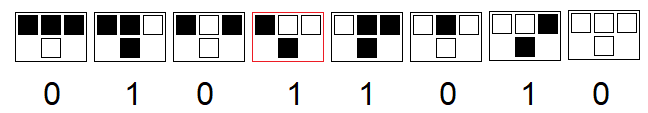
\includegraphics{image2.png}
    \caption{The next state of the center cell depends on the current state
    of a cell and its neighbors.}
    \label{fig:caRule}
\end{figure}

\pagebreak

As an example, let's look at the 4\textsuperscript{th} from left
arrangement, outlined in red. In the top row of this arrangement, the
center cell is dead and one of its neighbor's is alive.  Note that this
configuration has binary code 3'b100. Using the rule used to complete
Table~\ref{table:caNextState}, the next state of this cell is alive, shown black. The next
state value is placed below each configuration and the collection forms
an 8-bit number 8'b01011010, which when interpreted as a decimal value
is equal to 90. We will call the rule used to update the cells in Table
1, rule 90.

The fact that we are numbering this rule, implies that there may be
others. In fact, there are 256 different rule sets. You can create new
rules by substituting new combinations of alive and dead states for each
next states shown in Figure~\ref{fig:caRule}. Not all rules generate interesting
behavior. For example, rule 0 immediately kills any and all alive cells
producing a desert. Stephen Wolfram explored every combination of rules
and characterized the resulting patterns into one of four classes
depending on their sophistication. Wolfram illustrated this
sophistication by arranging successive iterations of the 1-DCA as rows.
As an example, if you start with a single alive cell and run Rule 90
over many iterations, drawing iteration below its predecessor, you get
the image shown in Figure~\ref{fig:caEvolution}. Some of you may recognize this figure as
the Sierpiński Triangle\footnote{\url{https://en.wikipedia.org/wiki/Sierpi\%C5\%84ski_triangle}},
an elementary fractal.

\begin{figure}[ht]
    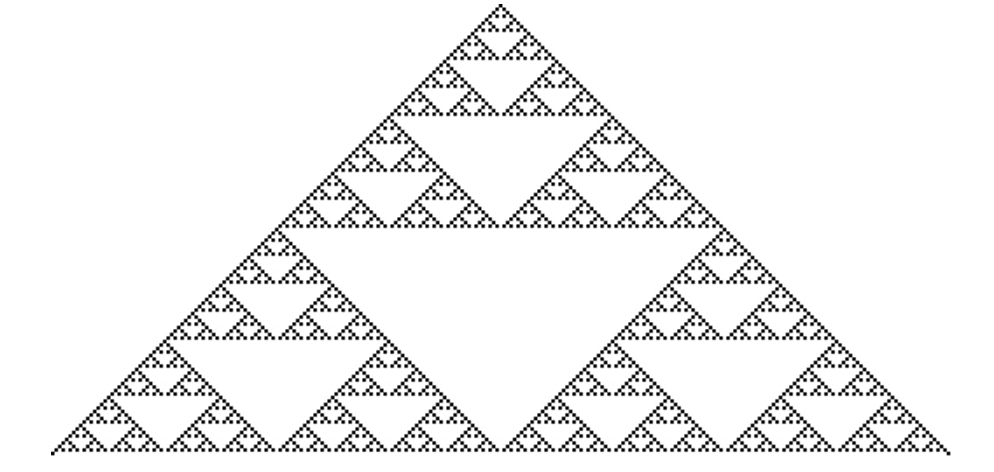
\includegraphics[width=0.5\paperwidth]{image3.png}
    \caption{The evolution of a single alive cell (shown at top) under Rule 90.}
    \label{fig:caEvolution}
\end{figure}

You now have all the information and terminology you need to build a
digital system to compute the next state of a 1-DCA, so let's get to it.

\subsection{Implementation: Cellular Automata}

You will use the inputs and outputs shown in Figure~\ref{fig:caDevBoard} to realize a
9 cell 1-DCA. I chose 9 cells so that we could have a unique center
cell. Each of the 9 \textbf{Initial State} slide switches corresponds to
one of the 9 cells. In order to set the state of the cells the
\textbf{loadRun} slide switch must be in the down position. Moving the
Initial State up/down will set its corresponding cell to 1/0
respectively when the array is clocked. A cell that is alive will
illuminate its associated \textbf{CurrentState} LED. After the initial
state of the cells is set, you should move the \textbf{loadRun} slide
switch up and set the 8-bit rule value using the \textbf{Rule} slide
switches. Every time that the array is clocked, the
\textbf{CurrentState} LEDs will show the array.

\begin{figure}[ht]
    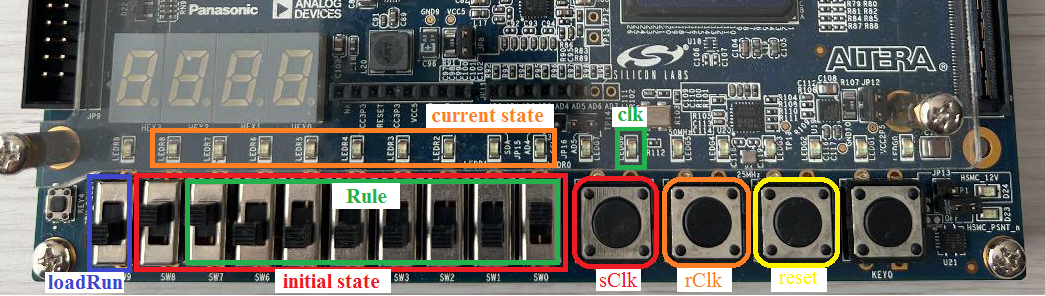
\includegraphics{image4.png}
    \caption{The input and output of the 1D cellular automata.}
    \label{fig:caDevBoard}
\end{figure}

The \textbf{reset} button will reset the state of all the cells to 0 --
dead. The clock is a bit more complex than you might expect because of
switch bouncing. When you press one of the push buttons on the Cyclone V
GX board, the signal generated may not transition smoothly from logic 0
to logic 1. Instead, it may do something like that shown in Figure~\ref{fig:caSwitchBounce}. In
this figure, a single press of the button created four transitions from
logic 0 to logic 1. This happens because the metal contact attached to
the round plastic button physically bounced off the metal contacts
attached to the body of the button. This is more prone to happen if you
quickly and sharply jab at the button.

\begin{figure}[ht]
    \begin{tabular}{ccc }
        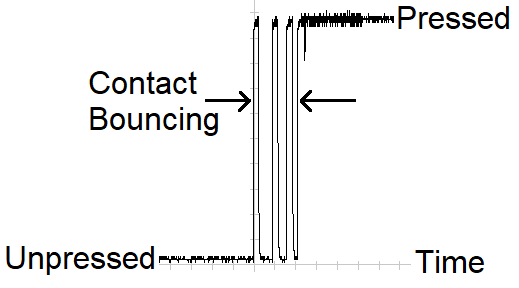
\includegraphics[width=0.3\paperwidth]{image5.png} &  & 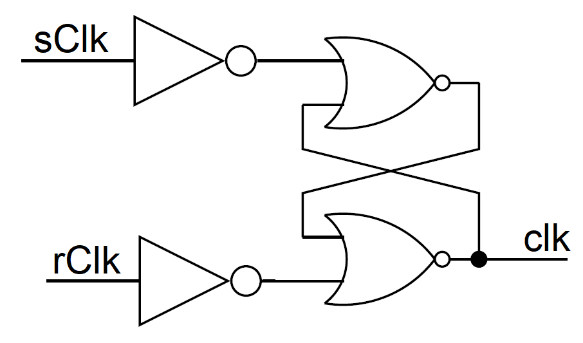
\includegraphics{image6.png} \\
        A  & & B \\
    \end{tabular}
    \caption{A) Switch bouncing makes generating a single clock edge problematic.
B) The organization of the SR latch to run the clock requires
inverters in the sClk and rClk inputs and an SR latch to help remove
signal bouncing.}
\label{fig:caSwitchBounce}
\end{figure}

However, even the most casual of presses may generate switch bouncing,
so you are going to design a digital circuit (an SR latch) to prevent
this from happening. When you press the \textbf{sClk} button, the clock
signal will be set. When you press the \textbf{rClk} button, the clk
signal will be reset. If the \textbf{sClk} or bounces, the clock line
will not bounce because this switch bounce will only cause the clk line
to be repeatedly be set when it already set. Likewise, with the
\textbf{rClk} signal repeatedly resetting the clk signal if
\textbf{rClk} bounces. Finally, in order for you to know the state of
the clk, its logic level is display on the \textbf{clk} LED.

Since the buttons driving the rClk and sClk signals are logic 0 when
pressed, you will want to invert these two signals before feeding them
into the SR latch as shown in Figure~\ref{fig:caSwitchBounce}B. Thus, to
toggle the clock signal
you will press/release the sClk button to set clk to 1. Then
press/release the rClk button to clear the clk to 0. The back to sClk,
etc\ldots{}

\section{System Architecture}

The system architecture shown in Figure~\ref{fig:caSysArch} shows the overall organization
of the cellular automata. Slide switches {[}0-7{]} are used as initial
state when the loadRun slide switch is set to 0. When the loadRun slide
switch is set to 1, slide switches {[}0-7{]} are used as the evolution
rule. The clock is generated by the SR latch whose inputs are sClk and
rClk. The state of the cells are displayed on the 9 red LEDs. The
processing elements forming the array are called singleCell and
discussed in the next section.

\begin{figure}[ht]
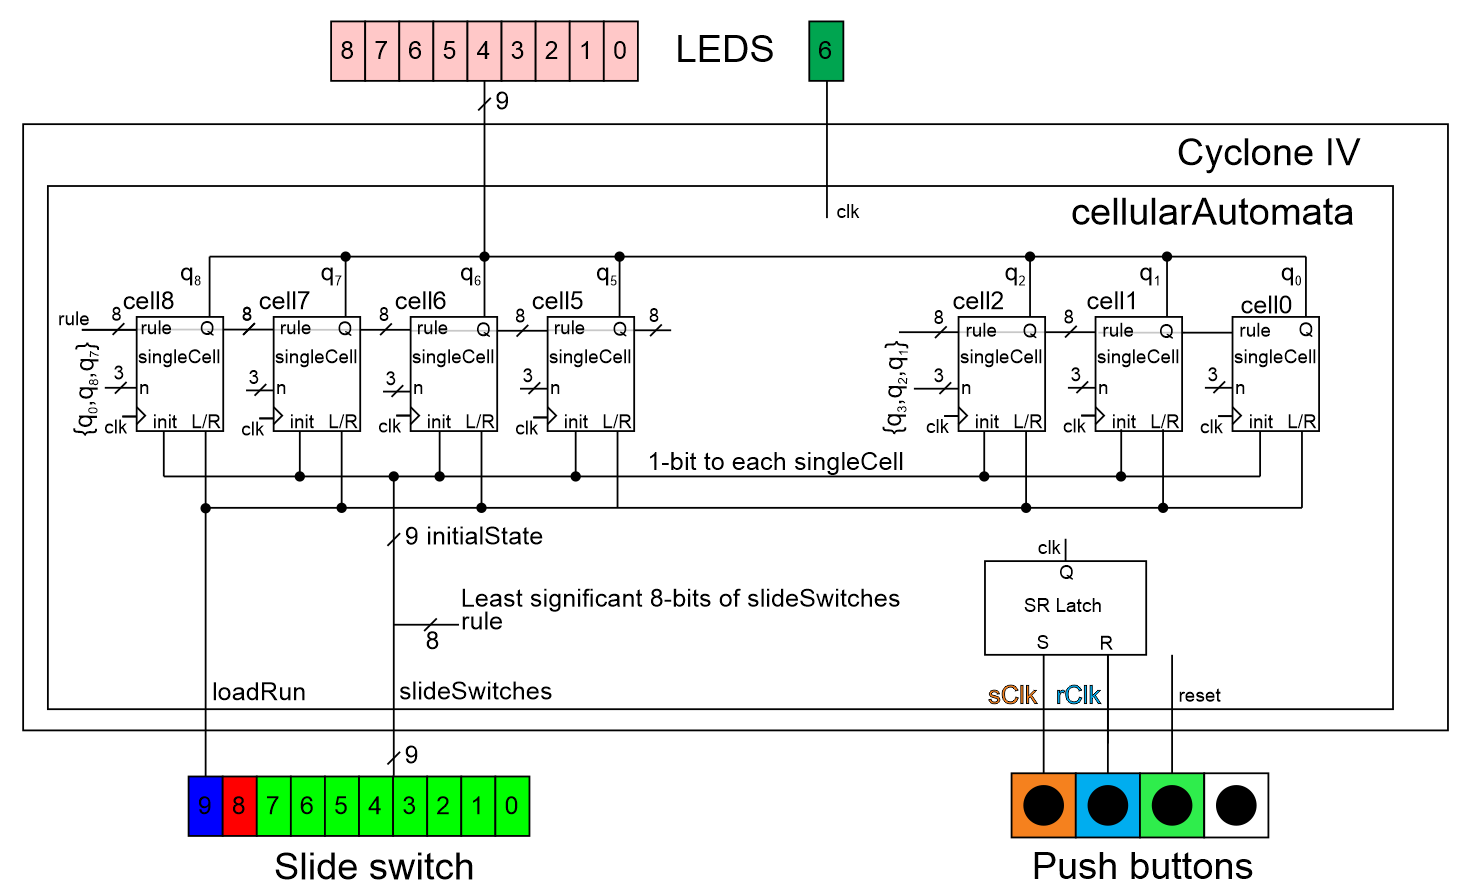
\includegraphics{image7.png}
\caption{The system architecture of the cellularAutomata. Due to tight
spacing, only the n inputs to cell8 and cell2 are shown.}
\label{fig:caSysArch}
\end{figure}

\protect\hypertarget{cellularAutomata_verilog}{}{}The Verilog code for
the cellularAutomata has been partially provided to you. You will need
to complete the missing pieces. For this module:

\begin{itemize}
\item
Use the cellularAutomata.v file provided in the Canvas folder as the
starting point.
\item
Make a vector for the \emph{rule} and \emph{initialState} from the
\emph{slideSwitches} input vector.
\item
Make a 3-bit vector input for each singleCell by appending its current
state to the two neighbors current state using the ``\{\}'' operators.
See the singleCell module for more information.
\item
Connect the ends of the CA together

\begin{itemize}
    \item
        Make cell 8 have cell 0 as its ``left'' neighbor in Figure~\ref{fig:caSysArch}
    \item
        Make cell 0 have cell 8 as its ``right'' neighbor in Figure~\ref{fig:caSysArch}
\end{itemize}
\item
Use cross-couples NORs and a pair of inverters to realize the SR-latch. This means that you
should have two lines of Verilog Code for the SR-latch, both starting
with ``assign''.
\item
You are encouraged to use the generate statement to instantiate
singleCell 1-7. Due the ring architecture, you will need to
instantiate cells 0 and 7 individually. For an example of the generate
statement, look at the adderSubtractor provided to you in a previous
lab.
\end{itemize}

\section{Module: singleCell}

The significant design problem in today's lab comes in this section,
building the singleCell module. The module interface for the singleCell
module in Figure~\ref{fig:caSysArch} used some shorthand for the single names due to the
space constraints. The internal organization and module interface for
the singleCell module is shown in Figure~\ref{fig:caSingleCell}. For example, the output
currentState in this figure was called Q in Figure~\ref{fig:caSysArch}. You should be able
to decipher the rest of the signal abbreviations used in Figure~\ref{fig:caSysArch}.

\begin{figure}[ht]
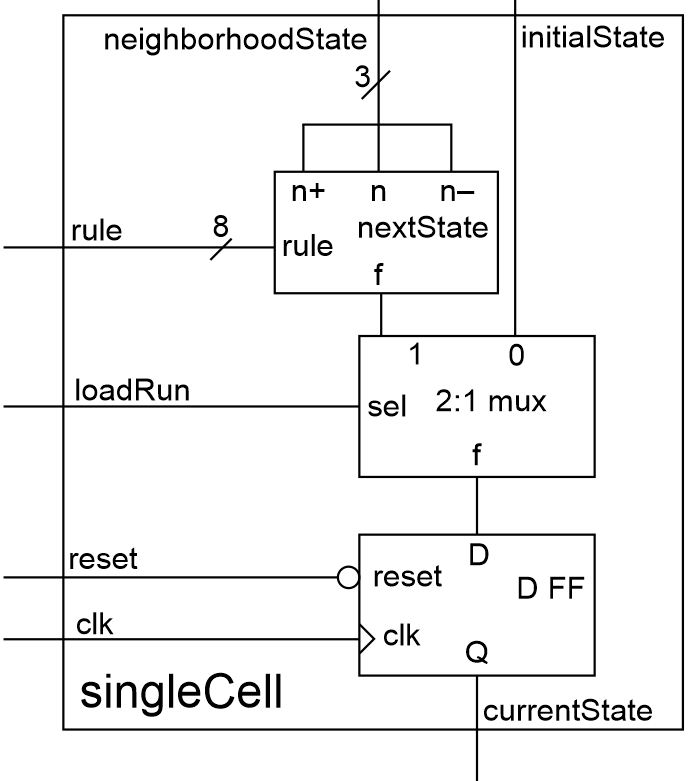
\includegraphics[width=0.3\paperwidth]{image8.png}
\caption{The architecture and module interface for the singleCell module.}
\label{fig:caSingleCell}
\end{figure}

The most complex portion of logic in the singleCell module is the box
labeled ``nextState''. This circuit has 11-bits of input.  While it may
seem a bit daunting at first, the Verilog code to realize this function
is pretty straightforward when you have the right perspective. Table~\ref{table:caInOutSingleCell}
lists all the combination of state for a cell and its 2 neighbors in the
left column (n+ is the state of the neighbor to the left, n the state of
the cell itself, and n- the state to the right). These 8 combinations
are the case values in the always/case statement for the nextState
logic. You need to know the output for each of these cases. As an
example, complete the nextState column in Table~\ref{table:caInOutSingleCell} for Rule 90 using the
information in Figure~\ref{fig:caRule}. In the ``Rule bit'' column in Table~\ref{table:caInOutSingleCell},
generalize the nextState column to the bit values in the 8-bit rule
vector that is passed into the singleCell module.

\begin{longtable}[]{@{}
| >{\raggedright\arraybackslash}p{(\columnwidth - 4\tabcolsep) * \real{0.3528}}|
>{\raggedright\arraybackslash}p{(\columnwidth - 4\tabcolsep) * \real{0.3236}}|
>{\raggedright\arraybackslash}p{(\columnwidth - 4\tabcolsep) * \real{0.3236}}|@{}}
\caption{The input/output relationship for the nextState
functionality in Figure~\ref{fig:caSingleCell}.}\label{table:caInOutSingleCell}\\ \hline
\toprule()
\{n+, n, n-\} &  nextState & Rule bit \\
\midrule()
\endfirsthead
\toprule()
\{n+, n, n-\} &  nextState & Rule bit \\
\midrule()
\endhead
3'b000 & & \\ \hline
3'b001 & & \\ \hline
3'b010 & & rule{[}2{]} \\ \hline
3'b011 & & \\ \hline
3'b100 & 1 & \\ \hline
3'b101 & & \\ \hline
3'b110 & & \\ \hline
3'b111 & & \\
\bottomrule()
\end{longtable}

\protect\hypertarget{singleCell_verilog}{}{}For the singleCell module, I
want you to:

\begin{itemize}
\item
Use the singleCell.v file provided in the Canvas folder as the
starting point.
\item
Use an always/case statement for the nextState logic
\item
Use the module definitions for:

\begin{itemize}
    \item
        Use the genericMux2x1 from a previous lab.
    \item
        Use the dffNegEdge module provided in the Canvas lab folder for this
        lab.
\end{itemize}
\item
Provide meaningful names to the wires in the module.
\item
Properly tab-indent your code

\begin{itemize}
    \item
        Single level for wire declarations
    \item
        Single level for component instantiations
    \item
        Two levels for case statement
    \item
        Three levels for case values
\end{itemize}
\end{itemize}

\section{Testbench}
\label{section:caTestbench}

Run the testbench for the cellularAutomata module provided on Canvas.
Produce a timing diagram with the following characteristics. Zoom to
fill the available horizontal space with the waveform. Color inputs
green and outputs red. Order the traces from top to bottom as

\begin{tabular}{p{4cm}p{4cm}p{4cm}}
signal        & radix                & tracel color \\ \hline
reset             & default             & Blue  \\
rule             &  unsigned             & Blue \\
sButton             & default         & Green \\
rButton             & default         & Green \\
clk                 & default         & Yellow \\
currentLifeState     & hex             & Red \\
\end{tabular}

Do not use the signals from the testbench, but rather the signals
from inside the cellularAutomata module. You can do this in ModelSim, by
expanding the cellularAutomata\_tb instance in the left ModelSim and
selecting ``uut''. Since uut is an instance of the cellularAutomata
module, all the signals accessible in the cellularAutomata module are
shown in the center Object. You can add signals using a drag-and-drop
operation. Likewise, you can reorder the signals by dragging them. Your
completed timing diagram should look something like Figure~\ref{fig:caTimeDiag}.

\begin{figure}[ht]
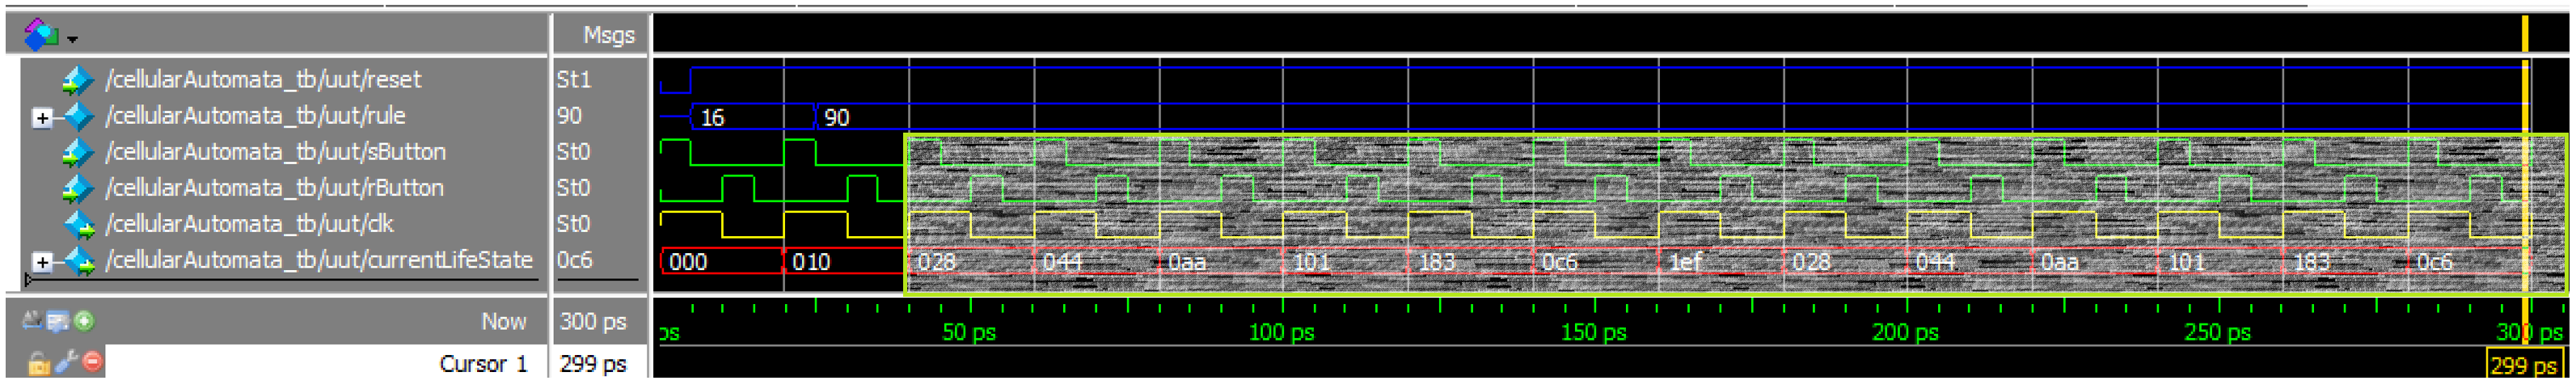
\includegraphics{image9.png}
\caption{Partial timing diagram for the cellular automata.}
\label{fig:caTimeDiag}
\end{figure}

\section{Pin-Assignment and Synthesis}

Use the image of the FPGA Board in Figure~\ref{fig:exampleCA}
and the information
in the C5G User Guide to determine the FPGA pins associated
with the input and output devices used by the cellular automata module.

\begin{longtable}[]{@{}
| >{\raggedright\arraybackslash}p{(\columnwidth - 8\tabcolsep) * \real{0.1986}}|
>{\raggedright\arraybackslash}p{(\columnwidth - 8\tabcolsep) * \real{0.2067}}|
>{\raggedright\arraybackslash}p{(\columnwidth - 8\tabcolsep) * \real{0.1935}}|
>{\raggedright\arraybackslash}p{(\columnwidth - 8\tabcolsep) * \real{0.1954}}|
>{\raggedright\arraybackslash}p{(\columnwidth - 8\tabcolsep) * \real{0.2058}}|@{}}
\caption{Pin Assignment for the 1-D calllular automata.}\label{table:cAutomataPinAssignment} \\ \hline
\endfirsthead
slide{[}9{]} & AE19 & &
Clk

LEDG6 & \\ \hline
slide{[}8{]} & & & led {[}8{]}

LEDR8 & \\ \hline
slide{[}7{]} & & & led {[}7{]} & K8\\ \hline
slide{[}6{]} & & & led {[}6{]} & \\ \hline
slide{[}5{]} & & & led {[}5{]} & \\ \hline
slide{[}4{]} & & & led {[}4{]} & \\ \hline
slide{[}3{]} & & & led {[}3{]} & \\ \hline
slide{[}2{]} & & & led {[}2{]} & \\ \hline
slide{[}1{]} & & & led {[}1{]} & \\ \hline
slide{[}0{]} & & & led {[}0{]}

LEDR0 & \\
\bottomrule()
\end{longtable}

\begin{longtable}[]{@{}
| >{\raggedright\arraybackslash}p{(\columnwidth - 4\tabcolsep) * \real{0.3334}}|
>{\raggedright\arraybackslash}p{(\columnwidth - 4\tabcolsep) * \real{0.3334}}|
>{\raggedright\arraybackslash}p{(\columnwidth - 4\tabcolsep) * \real{0.3333}}|@{}}
\toprule()
\begin{minipage}[b]{\linewidth}\raggedright
sClk
\end{minipage} &
\begin{minipage}[b]{\linewidth}\raggedright
Key{[}3{]}
\end{minipage} &
\begin{minipage}[b]{\linewidth}\raggedright
\end{minipage} \\
\midrule()
\endhead
\begin{minipage}[t]{\linewidth}\raggedright
rClk
\end{minipage} & Key{[}2{]} & Y15 \\ \hline
\begin{minipage}[t]{\linewidth}\raggedright
reset
\end{minipage} & Key{[}1{]} & \\
\bottomrule()
\end{longtable}

Complete the pin-assignment in Quartus, compile your design and download to the
FGPA development boards.  If you are having difficulty getting your circuit to work
correctly, please refer to Section~\ref{section:caDebugging} for some
useful debugging tips.

Once you get your design working, demonstrate it to a member of the
lab team.

\section{Turn in}

You may work in teams of at most two. Make a record of your response to
the items below and turn them in a single copy as your team's solution
on Canvas using the instructions posted there. Include the names of both
team members at the top of your solutions. Use complete English
sentences to introduce what each of the following listed items (below)
is and how it was derived. In addition to this submission, you will be
expected to demonstrate your circuit at the beginning of your lab
section next week.

\subsubsection{Cellular Automata Module }

\begin{itemize}
\item
Complete Table~\ref{table:caNextState}.
\item
\protect\hyperlink{cellularAutomata_verilog}{Link} Verilog code for
the body of the cellularAutomata module (courier 8-point font single
spaced), leave out header comments.
\end{itemize}

\subsubsection{singleCell Module}

\begin{itemize}
\item
Complete Table~\ref{table:caInOutSingleCell}.
\item
\protect\hyperlink{singleCell_verilog}{Link} Verilog code for the body
of the singleCell module (courier 8-point font single spaced), leave
out header comments.
\end{itemize}

\subsubsection{Testbench}
\begin{itemize}
\item Complete testbench and timing diagram from Section~\ref{section:caTestbench}.
\end{itemize}

\subsubsection{Pin-Assignment and Synthesis}
\begin{itemize}
\item Complete the pin assignment in table~\ref{table:cAutomataPinAssignment}.
\item Demonstrate your completed circuit to a lab team member.
\end{itemize}

\section{Debugging Tips}
\label{section:caDebugging}
To provide you with some examples to run on the Altera boards, the
following table illustrates the evolution of the CA with different
initial conditions and different rules.

\begin{itemize}
\item
In the left most column contains several different rows

\begin{itemize}
    \item
        The row labeled ``Rule \#'' is the rule that you will enter on the
        slide switches. The binary code of the rule is provided to make
        setting your dip switches easier.
    \item
        The row labeled ``start'' is the initial load value stored in the
        CA. A value of ``x'' means that the initial load value doesn't
        matter (don't care).
    \item
        The rows labeled ``iteration'' count successive positive edges
        generated by the clock.
\end{itemize}
\item
The column labeled
``q\textsubscript{8}q\textsubscript{7}q\textsubscript{6}q\textsubscript{5}''
is the output from the 4 most significant bits of the CA
\item
The column labeled ``q\textsubscript{4}'' is the output from the
middle bit of the CA
\item
The column labeled
``q\textsubscript{3}q\textsubscript{2}q\textsubscript{1}q\textsubscript{0}''
is the output from the 4 least significant bits of the CA
\end{itemize}

\begin{longtable}[]{@{}
|  >{\raggedright\arraybackslash}p{(\columnwidth - 6\tabcolsep) * \real{0.2723}}|
>{\raggedright\arraybackslash}p{(\columnwidth - 6\tabcolsep) * \real{0.2426}}|
>{\raggedright\arraybackslash}p{(\columnwidth - 6\tabcolsep) * \real{0.2426}}|
>{\raggedright\arraybackslash}p{(\columnwidth - 6\tabcolsep) * \real{0.2426}}|@{}} \\ \hline
\endfirsthead
\endhead

\textbf{Rule 0:}

\textbf{0000 0000}  &  q\textsubscript{8}q\textsubscript{7}q\textsubscript{6}q\textsubscript{5}
& q\textsubscript{4} & q\textsubscript{3}q\textsubscript{2}q\textsubscript{1}q\textsubscript{0} \\ \hline
Start: & XXXX & X & XXXX \\ \hline
Final: & 0000 & 0 & 0000 \\ \hline
& & & \\ \hline
\textbf{Rule 255:}

\textbf{1111 1111} & & & \\ \hline
Start: & XXXX & X & XXXX \\ \hline
Final: & 1111 & 1 & 1111 \\ \hline
& & & \\ \hline
\textbf{Rule 90:}

\textbf{0101 1010} & & & \\ \hline
Start: & 0000 & 1 & 0000 \\ \hline
1st Iteration: & 0001 & 0 & 1000 \\ \hline
2nd Iteration: & 0010 & 0 & 0100 \\ \hline
3rd Iteration: & 0101 & 0 & 1010 \\ \hline
4th Iteration: & 1000 & 0 & 0001 \\ \hline
5th Iteration & 1100 & 0 & 0011 \\ \hline
6th Iteration & 0110 & 0 & 0110 \\ \hline
7th Iteration & 1111 & 0 & 1111 \\ \hline
& & & \\ \hline
\textbf{Rule 90:}

\textbf{0101 1010} & & & \\ \hline
Start: & 1011 & 0 & 1101 \\ \hline
1st Iteration: & 1011 & 0 & 1101 \\ \hline
Final: & 1011 & 0 & 1101 \\ \hline
& & & \\ \hline
\textbf{Rule 254:}

\textbf{1111 1110} & & 1111 & 1110 \\ \hline
Start: & 1000 & 0 & 0000 \\ \hline
1st Iteration: & 1100 & 0 & 0001 \\ \hline
2nd Iteration: & 1110 & 0 & 0011 \\ \hline
3rd Iteration: & 1111 & 0 & 0111 \\ \hline
Final: & 1111 & 1 & 1111 \\
\bottomrule()
\end{longtable}
